 \documentclass[12pt,a4paper]{article}
%\usepackage{hyperref} % Use the Charter font for the document text
%\usepackage[UTF8]{ctex}
\usepackage{jheppub}

\usepackage{amsfonts,amssymb,amsmath}
\usepackage{mathtools}
\usepackage{tikz-cd}
\usepackage{tikz}
\usepackage{alltt}
\usepackage{amsfonts}
\usepackage{amsmath}
\usepackage{amssymb}
\usepackage{amsthm}
\usepackage{booktabs}
\usepackage{caption}
\usepackage{enumitem}
\usepackage{fancyhdr}
\usepackage{graphicx}
\usepackage{mathdots}
\usepackage{mathtools}
\usepackage{microtype}
\usepackage{multirow}
\usepackage{pdflscape}
\usepackage{pgfplots}
\usepackage{siunitx}
\usepackage{slashed}
\usepackage{tabularx}
\usepackage{tikz}
\usepackage{tkz-euclide}
\usepackage[normalem]{ulem}
\usepackage[all]{xy}
\usepackage{imakeidx}

\usepackage{wrapfig}



%%%%%%%  Greek letters %%%%%%%%%%%%%%%%%%
\def\a{\alpha}
\def\b{\beta}
\def\c{\gamma} \def\g{\gamma}
\def\d{\delta}
\def\e{\epsilon}
\def\f{\phi}
\def\vf{\varphi}  \def\tvf{\tilde{\varphi}}
\def\vp{\varphi}
\def\h{\eta}
\def\i{\iota}
\def\j{\psi}
\def\k{\kappa}
\def\m{\mu}
\def\n{\nu}
\def\o{\omega}  \def\w{\omega}
\def\q{\theta}  \def\th{\theta}
\def\r{\rho}
\def\s{\sigma}
\def\t{\tau}
\def\u{\upsilon}
\def\x{\xi}
\def\z{\zeta}

\def\A{\Alpha}
\def\B{\Beta}
\def\G{\Gamma}
\def\D{\Delta}
\def\E{\Epsilon}
\def\F{Phi}
\def\h{\eta}
\def\I{\Iota}
\def\J{Psi}
\def\K{\Kappa}
\def\L{\Lambda}
\def\M{\Mu}
\def\N{\Nu}
\def\O{\Omega}  \def\w{\omega}
\def\Q{\Theta}  \def\Th{\Theta}
\def\R{\Rho}
\def\Si{\Sigma}
\def\T{\Tau}
\def\Up{\Upsilon}
\def\X{\Xi}
\def\Z{\Zeta}








%%%%%%%%%%%% math fonts %%%%%%%%%%%%%%%%%%%%%%%%%%%%%%%%%%%%%
%
%---------- mathbb font --------------------------------
%

\newcommand{\bA}{\ensuremath{\mathbb{A}}}
\newcommand{\bB}{\ensuremath{\mathbb{B}}}
\newcommand{\bC}{\ensuremath{\mathbb{C}}}
\newcommand{\bD}{\ensuremath{\mathbb{D}}}
\newcommand{\bE}{\ensuremath{\mathbb{E}}}
\newcommand{\bF}{\ensuremath{\mathbb{F}}}
\newcommand{\bG}{\ensuremath{\mathbb{G}}}
\newcommand{\bH}{\ensuremath{\mathbb{H}}}
\newcommand{\bI}{\ensuremath{\mathbb{I}}}
\newcommand{\bJ}{\ensuremath{\mathbb{J}}}
\newcommand{\bK}{\ensuremath{\mathbb{K}}}
\newcommand{\bL}{\ensuremath{\mathbb{L}}}
\newcommand{\bM}{\ensuremath{\mathbb{M}}}
\newcommand{\bN}{\ensuremath{\mathbb{N}}}
\newcommand{\bO}{\ensuremath{\mathbb{O}}}
\newcommand{\bP}{\ensuremath{\mathbb{P}}}
\newcommand{\bQ}{\ensuremath{\mathbb{Q}}}
\newcommand{\bR}{\ensuremath{\mathbb{R}}}
\newcommand{\bS}{\ensuremath{\mathbb{S}}}
\newcommand{\bT}{\ensuremath{\mathbb{T}}}
\newcommand{\bU}{\ensuremath{\mathbb{U}}}
\newcommand{\bV}{\ensuremath{\mathbb{V}}}
\newcommand{\bW}{\ensuremath{\mathbb{W}}}
\newcommand{\bX}{\ensuremath{\mathbb{X}}}
\newcommand{\bY}{\ensuremath{\mathbb{Y}}}
\newcommand{\bZ}{\ensuremath{\mathbb{Z}}}


%
%\parskip=1em
%\parindent=0.3in
%\setlength\oddsidemargin{0.5in} \setlength\evensidemargin{0.5in}
%\setlength\textwidth{5.5in}
%
%\hfuzz6pt % Don't bother to report over-full boxes if over-edge is < 6pt
%
%\newlength{\defbaselineskip}
%\setlength{\defbaselineskip}{\baselineskip}
%\newcommand{\setlinespacing}[1]%
%           {\setlength{\baselineskip}{#1 \defbaselineskip}}
%\newcommand{\doublespacing}{\setlength{\baselineskip}%
%                           {2.0 \defbaselineskip}}
%\newcommand{\singlespacing}{\setlength{\baselineskip}{\defbaselineskip}}
%
%\newcommand{\properpagestyle}{\pagestyle{myheadings}\markboth{}{}\markright{}}


%---------- mathscript font -----------------------------
%

\newcommand{\scA}{\ensuremath{\mathscr{A}}}
\newcommand{\scB}{\ensuremath{\mathscr{B}}}
\newcommand{\scC}{\ensuremath{\mathscr{C}}}
\newcommand{\scD}{\ensuremath{\mathscr{D}}}
\newcommand{\scE}{\ensuremath{\mathscr{E}}}
\newcommand{\scF}{\ensuremath{\mathscr{F}}}
\newcommand{\scG}{\ensuremath{\mathscr{G}}}
\newcommand{\scH}{\ensuremath{\mathscr{H}}}
\newcommand{\scI}{\ensuremath{\mathscr{I}}}
\newcommand{\scJ}{\ensuremath{\mathscr{J}}}
\newcommand{\scK}{\ensuremath{\mathscr{K}}}
\newcommand{\scL}{\ensuremath{\mathscr{L}}}
\newcommand{\scM}{\ensuremath{\mathscr{M}}}
\newcommand{\scN}{\ensuremath{\mathscr{N}}}
\newcommand{\scO}{\ensuremath{\mathscr{O}}}
\newcommand{\scP}{\ensuremath{\mathscr{P}}}
\newcommand{\scQ}{\ensuremath{\mathscr{Q}}}
\newcommand{\scR}{\ensuremath{\mathscr{R}}}
\newcommand{\scS}{\ensuremath{\mathscr{S}}}
\newcommand{\scT}{\ensuremath{\mathscr{T}}}
\newcommand{\scU}{\ensuremath{\mathscr{U}}}
\newcommand{\scV}{\ensuremath{\mathscr{V}}}
\newcommand{\scW}{\ensuremath{\mathscr{W}}}
\newcommand{\scX}{\ensuremath{\mathscr{X}}}
\newcommand{\scY}{\ensuremath{\mathscr{Y}}}
\newcommand{\scZ}{\ensuremath{\mathscr{Z}}}
\newcommand{\scAH}{\ensuremath{\mathscr{A}\!\!\scH}}

%
%---------- mathfrak font -----------------------------
%

\newcommand{\frakA}{\ensuremath{\mathfrak{A}}}
\newcommand{\frakB}{\ensuremath{\mathfrak{B}}}
\newcommand{\frakC}{\ensuremath{\mathfrak{C}}}
\newcommand{\frakD}{\ensuremath{\mathfrak{D}}}
\newcommand{\frakE}{\ensuremath{\mathfrak{E}}}
\newcommand{\frakF}{\ensuremath{\mathfrak{F}}}
\newcommand{\frakG}{\ensuremath{\mathfrak{G}}}
\newcommand{\frakH}{\ensuremath{\mathfrak{H}}}
\newcommand{\frakI}{\ensuremath{\mathfrak{I}}}
\newcommand{\frakJ}{\ensuremath{\mathfrak{J}}}
\newcommand{\frakK}{\ensuremath{\mathfrak{K}}}
\newcommand{\frakL}{\ensuremath{\mathfrak{L}}}
\newcommand{\frakM}{\ensuremath{\mathfrak{M}}}
\newcommand{\frakN}{\ensuremath{\mathfrak{N}}}
\newcommand{\frakO}{\ensuremath{\mathfrak{O}}}
\newcommand{\frakP}{\ensuremath{\mathfrak{P}}}
\newcommand{\frakQ}{\ensuremath{\mathfrak{Q}}}
\newcommand{\frakR}{\ensuremath{\mathfrak{R}}}
\newcommand{\frakS}{\ensuremath{\mathfrak{S}}}
\newcommand{\frakT}{\ensuremath{\mathfrak{T}}}
\newcommand{\frakU}{\ensuremath{\mathfrak{U}}}
\newcommand{\frakV}{\ensuremath{\mathfrak{V}}}
\newcommand{\frakW}{\ensuremath{\mathfrak{W}}}
\newcommand{\frakX}{\ensuremath{\mathfrak{X}}}
\newcommand{\frakY}{\ensuremath{\mathfrak{Y}}}
\newcommand{\frakZ}{\ensuremath{\mathfrak{Z}}}
\newcommand{\fraka}{\ensuremath{\mathfrak{a}}}
\newcommand{\frakb}{\ensuremath{\mathfrak{b}}}
\newcommand{\frakc}{\ensuremath{\mathfrak{c}}}
\newcommand{\frakd}{\ensuremath{\mathfrak{d}}}
\newcommand{\frake}{\ensuremath{\mathfrak{e}}}
\newcommand{\frakf}{\ensuremath{\mathfrak{f}}}
\newcommand{\frakg}{\ensuremath{\mathfrak{g}}}
\newcommand{\frakh}{\ensuremath{\mathfrak{h}}}
\newcommand{\fraki}{\ensuremath{\mathfrak{i}}}
\newcommand{\frakj}{\ensuremath{\mathfrak{j}}}
\newcommand{\frakk}{\ensuremath{\mathfrak{k}}}
\newcommand{\frakl}{\ensuremath{\mathfrak{l}}}
\newcommand{\frakm}{\ensuremath{\mathfrak{m}}}
\newcommand{\frakn}{\ensuremath{\mathfrak{n}}}
\newcommand{\frako}{\ensuremath{\mathfrak{o}}}
\newcommand{\frakp}{\ensuremath{\mathfrak{p}}}
\newcommand{\frakq}{\ensuremath{\mathfrak{q}}}
\newcommand{\frakr}{\ensuremath{\mathfrak{r}}}
\newcommand{\fraks}{\ensuremath{\mathfrak{s}}}
\newcommand{\frakt}{\ensuremath{\mathfrak{t}}}
\newcommand{\fraku}{\ensuremath{\mathfrak{u}}}
\newcommand{\frakv}{\ensuremath{\mathfrak{v}}}
\newcommand{\frakw}{\ensuremath{\mathfrak{w}}}
\newcommand{\frakx}{\ensuremath{\mathfrak{x}}}
\newcommand{\fraky}{\ensuremath{\mathfrak{y}}}
\newcommand{\frakz}{\ensuremath{\mathfrak{z}}}
\newcommand{\fraksl}{\ensuremath{\mathfrak{sl}}}
\newcommand{\frakso}{\ensuremath{\mathfrak{so}}}
\newcommand{\fraksp}{\ensuremath{\mathfrak{sp}}}

%%%%%%%%%%%%  Calligraphic, Roman and Maths integers %%%%%%%%%%%%%%%%%%

\newcommand{\cA}{\mathcal{A}}
\newcommand{\cB}{\mathcal{B}}
\newcommand{\cC}{\mathcal{C}}
\newcommand{\cD}{\mathcal{D}}
\newcommand{\cE}{\mathcal{E}}
\newcommand{\cF}{\mathcal{F}}
\newcommand{\cG}{\mathcal{G}}
\newcommand{\cH}{\mathcal{H}}
\newcommand{\cI}{\mathcal{I}}
\newcommand{\cJ}{\mathcal{J}}
\newcommand{\cK}{\mathcal{K}}
\newcommand{\cL}{\mathcal{L}}
\newcommand{\cM}{\mathcal{M}}
\newcommand{\cN}{\mathcal{N}}
\newcommand{\cO}{\mathcal{O}}
\newcommand{\cQ}{\mathcal{Q}}
\newcommand{\cS}{\mathcal{S}}
\newcommand{\cX}{\mathcal{X}}
\newcommand{\cY}{\mathcal{Y}}
\newcommand{\cW}{\mathcal{W}}
\newcommand{\cR}{\mathcal{R}}
\newcommand{\cT}{\mathcal{T}}
\newcommand{\cZ}{\mathcal{Z}}

%%%%%%%%%%%%%%%%%%%%%%%%%%%%%%%%%%%%%%%%%%%%%%%%%%%%%%%%%%%%%%%%
\newcommand{\SU}{\mathrm{SU}}
\newcommand{\SO}{\mathrm{SO}}
\newcommand{\SL}{\mathrm{SL}}
\newcommand{\Sp}{\mathrm{Sp}}
\newcommand{\su}{\mathrm{su}}
\newcommand{\so}{\mathrm{so}}
\newcommand{\spl}{\mathrm{sp}}
\newcommand{\gl}{\mathrm{gl}}
\newcommand{\sll}{\mathrm{sl}}
\newcommand{\U}{\mathrm{U}}
\newcommand{\ul}{\mathrm{u}}
\newcommand{\Spin}{\mathrm{Spin}}
\newcommand{\Pin}{\mathrm{Pin}}
%%%%%%%%%%%%%%%%%%%%%%%%%%%%%%%%%%%%%%%%%%%%%%%%%%%%%%%%%%%%%%%%
\renewcommand{\Im}{{\rm Im}}
\renewcommand{\Re}{{\rm Re}}
\newcommand{\Tr}{\mbox{Tr}}
\newcommand{\Pf}{\mbox{Pf}}
\newcommand{\sgn}{\mbox{sgn}}
\newcommand{\Vir}{{\rm Vir}}
\newcommand{\Li}{{\rm Li}}

\def\tl{\tilde}
\def\wt{\widetilde}
\def\wh{\widehat}
\def\bar{\overline}





\def\bea{\begin{align}}
\def\eea{\end{align}}
\def\be{\begin{equation}}
\def\ee{\end{equation}}
\def\ba{\begin{align}}
\def\ea{\end{align}}


%\title{ Lecture 4}
\begin{document}\thispagestyle{empty}

\centerline{\Large \bf  Lecture 1}

\section{Motivation and Overview}

\subsection{Why do we study string theory?}

$\bullet$ \textbf{For quantum gravity}


One of the major problems in theoretical physics is to provide unified description of all the forces in Nature. The standard model has unified electro-magnetic, weak and strong force based on quantum field theories whereas general relativity for gravity is formulated within the framework of classical physics. A quantum theory of gravity is needed in order to reconcile general relativity with the principles of quantum mechanics. However, it is known that the renormalization procedure does not cure ultraviolet divergence for gravity. Therefore, naive quantization of general relativity does not give a consistent theory.

String theory not only yields the first quantization of gravity but also resolves the renormalization problem of gravity by replacing point particles by vibrating strings.  To my knowledge, string theory is currently the only theory which has this property. Once we discover a candidate to unify gravity and quantum mechanics of all the forces, it is inevitable to try to understand it as well as we can although there is never any guarantee we can achieve.

Indeed, string theory has given deep insights about quantum gravity. The Beckenstein-Hawking formula \cite{Bekenstein:1973ur,Bardeen:1973gs,Hawking:1974sw} was microscopically derived by counting D-brane states with fixed mass and charge for certain (called extremal) black holes in string theory \cite{Strominger:1996sh}. The AdS/CFT correspondence \cite{Maldacena:1997re} conjectures that non-perturbative definition of a string theory on AdS background is described by a conformal field theory, and it partially resolves Hawking information paradox of black hole \cite{Hawking:1976ra}. Interestingly, a generalization of the Beckenstein-Hawking formula, called the Ryu-Takayanagi entanglement entropy formula \cite{Ryu:2006bv}, connects quantum gravity and quantum information theory, which is actively studied in recent years.\footnote{Ling-Yan Hung at Fudan has been working on this area.} These developments certainly pose questions to basic concepts of space-time.





\vspace{.3cm}



\begin{wrapfigure}{L}{0.5\textwidth}
\includegraphics[width=7cm]{M-Theory}
\end{wrapfigure}



\noindent$\bullet$ \textbf{Rich arena for physics theories}


String theory has shed a lot of light on the behavior of an established physical theory. These range from proof of positive energy, quark confinement, heavy iron collisions, quantum critical behavior, quantum black holes, quantum information, etc. Moreover it sometimes sets up a new framework to study established physical theory. In my opinion, there are two reasons for it. One reason is that string theory can generates vast families (in fact, infinitely many) of quantum field theories in various dimensions. There are five types of string theories, Type I, IIA, IIB, Heterotic $\SO(32)$, $E_8\times E_8$ and M-theory is a limit of large dilaton expectation value in Type IIA  string theory. In addition, Type II theories can contain D$p$-branes, and M-theory can have M2 and M5-branes. Although there are finitely many string theories, they can ``engineer'' infinitely many quantum field theories depending on manifolds string theory lives and brane configurations. The other reason is duality, an equivalence between two different descriptions at quantum level. In fact, string theories of five types are related by a web of dualities (see figure), and the AdS/CFT correspondence is another kind of duality. More dualities have been (and hopefully will be) discovered in string theories and a duality plays a crucial role to show drastically different viewpoint for established physical theory.

Through recent developments in string theory, especially in the study of M5-branes, we have learned that there are vast families of QFTs which do not admit Lagrangian description. They are intrinsically strongly-coupled so that techniques in QFT we have developed for decades cannot be used. Currently, we are trying to understand QFTs without Lagrangian description case by case by using dualities, dimensional reduction on some manifolds,  RG flows or perturbing theories. However, there is no consistent unified description for these theories, and we therefore need new framework to describe QFTs without Lagrangian description.


%
%There are many instances where questions are asked in the context of established physical theory. And often they are simply questions about known but intractable equations the standard physical theories where re-asking these questions in light of string theory has given us a lot more insights about the answers.

\vspace{.3cm}
\noindent$\bullet$ \textbf{For mathematical structure}

There is a certain group of people who are interested in string theory because it has brought about a lot of new insights in mathematics, especially in geometry.\footnote{Indeed I belong to this group.} String theory has repeatedly provided new ways to look at geometry, which arise as  inevitable consequences of trying to understand how physical theory should be. Mirror symmetry \cite{Candelas:1990rm}, Seiberg-Witten invariants \cite{Witten:1994cg}, AGT relation \cite{Alday:2009aq}, etc are salient examples. Moreover, string dualities have led highly non-trivial conjectures that connect seemingly different subjects of mathematics.  String theory provides  many insights in geometry partly because we do not understand the theory. In contrast to the fact that Einstein theory of gravity has been constructed based on Riemannian geometry, we do not understand geometric foundation for string theory yet.  However, physicists can come up with new insights in geometry because physicists stumble upon very deep theory we do not understand well. It is certain that there are more mathematical secrets in string theory.


\vspace{.3cm}
\noindent$\bullet$ \textbf{Because we do not know what it is}

As mentioned, we do not understand the core new concept string theory is base on, but we know it is remarkably rich.
One of the reason that string theory is an exciting topic to work on for students is precisely that so much things are not understood yet. It sometimes framed criticisms that string theorists do not understand the theory. That's true. But if we understood it, there would be ground-breaking insights both in physics and mathematics. The fact that so little is understood and such relatively small pieces are actually such big discoveries in its own right makes us exciting. Of course, there is still a lot more to do!

\subsection{Very very brief history}

String theory was invented originally by accident in trying to solve a different problem, subsequently developed by a long and fortunate process of tinkering. Therefore, the history of string theory itself is interesting. For detailed history of string theory, we refer to \cite{Greene:1999kj,Schwarz,Schwarz:2011ona,Ooguribook,Polchinski:2017vik}. \footnote{Yuji Tachikawa has recommended us a good book \cite{cappelli2012birth} that describes the early history of string theory more in detail. Thanks to Yuji!}

String theory was first developed by aiming at describing hadron physics. People came up an idea that a meson is a little string with charges at its end and the meson resonances are vibrational states of the string. Although this physical picture, which first emerged from the Veneziano amplitude \cite{Veneziano:1968yb}, is now believed to be qualitatively correct at a description of strongly interacting particles, QCD became far more successful to describe details of strong interactions soon later.

However, a small group of physicists has continued to study string theory in 70s and it was found that string theory includes massless spin-two particles, suggesting that string theory can be a theory of gravity. Furthermore, a tachyon which is present in bosonic string theory turned out to be absent by incorporating supersymmetry, and Type IIA and IIB as well as Type I theories have been constructed.

In 1984, Green and Schwarz showed \cite{Green:1984sg} that anomaly pointed out by Alvarez-Gaum\'e  and Witten is cancelled if the gauge group of Type I string theory is $\SO(32)$, which led to the first string revolution. A number of people has started working in the field of string theory. During the first revolution, Heterotic string theory has been constructed.

In 1995, Witten has proposed \cite{Witten:1995ex}  that five types of string theories are related by dualities and they are moreover five different limits of one bigger theory called M-theory. This has led to the second string revolution during which D-branes are proposed and non-perturbative aspects of string theories have been extensively studied. These results bore fruits as discoveries of a number of dualities, understanding of quantum nature of black holes and the AdS/CFT correspondence.

The second revolution has driven more researchers to study D-brane worldvolume theories and their relations to quantum gravity. However, dynamics on M2-branes and M5-branes that are fundamental degrees of freedoms in M-theory have remained elusive. Triggered by the work of Bagger-Lambert \cite{Bagger:2006sk}, the worldvolume theory for M2-branes was found to be a highly supersymmetric exquisite mixture of Chern-Simons gauge theory with some scalars and spinors \cite{Aharony:2008ug}. On the other hand, the worldvolume theory on M5-branes is difficult to analyze because it is known that it does not admit Lagrangian description. However, the paper of Gaiotto \cite{Gaiotto:2009we} has ignited the study of properties of M5-branes by wrapping them on a certain manifold, which still continues to be active so far.

The following picture shows the timeline of string theory and when the standard textbooks were written.\footnote{Of course, there are many other books \cite{Zwiebach:2004tj,Dine:2007zp,Ibanez:2012zz,Blumenhagen:2013fgp} and notes \cite{Uranga,Tong:2009np,wray2011introduction,Hosomichi,Weigand}.} Obviously, the textbooks do not cover developments after their publications. We will mainly use Polchinski's textbook \cite{Polchinski}, but I do not recommend to stick only on one book when you study a subject. In a book, some parts are explained very well, but some parts are sometimes hard to grasp for some people. Therefore, it is always a good idea to look for books, notes and papers that suit you best.
\begin{figure}[h]\centering
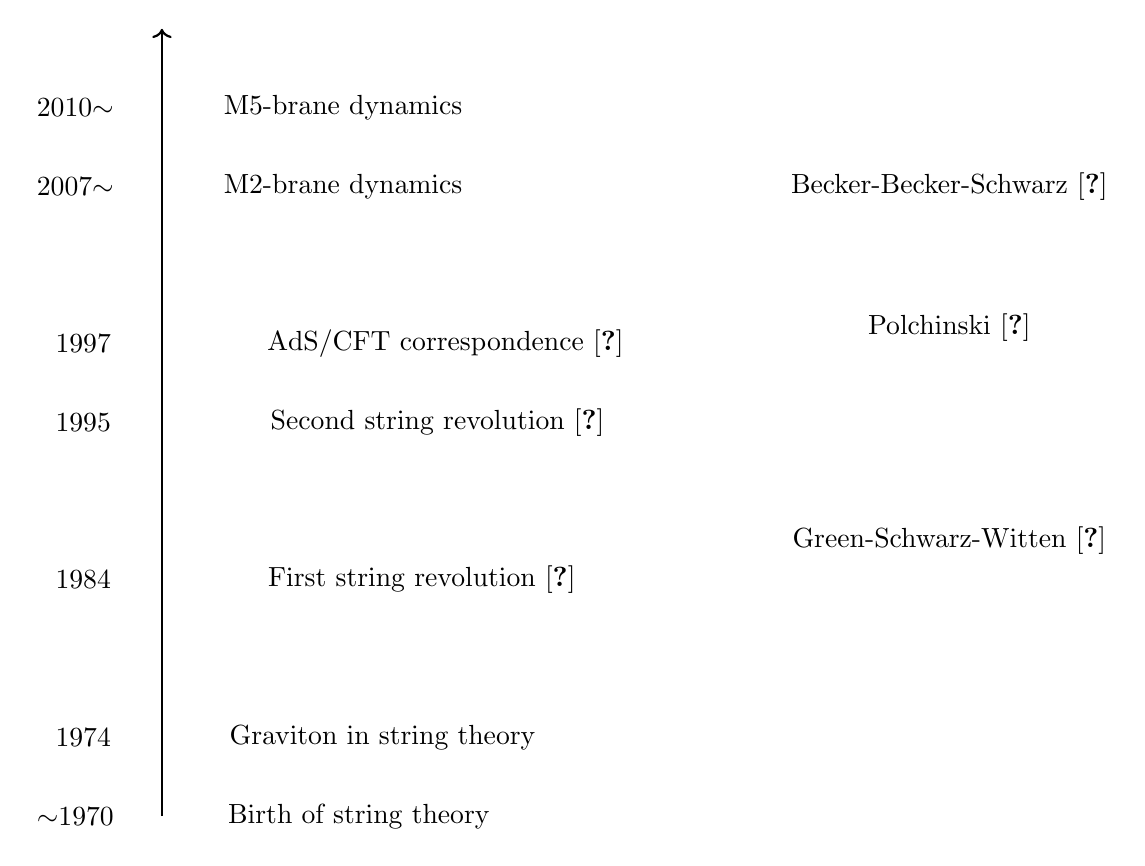
\begin{tikzpicture}
\draw[->,thick]  (0,0) to (0,10);
\node at  (2.3,9) {M5-brane dynamics};
\node at  (-1.1,9) {2010$\sim$};
\node at  (10,8) {Becker-Becker-Schwarz \cite{BBS}};
\node at  (2.3,8) {M2-brane dynamics};
\node at  (-1.1,8) {2007$\sim$};
\node at  (10,6.2) {Polchinski \cite{Polchinski}};
\node at  (3.6,6) {AdS/CFT correspondence \cite{Maldacena:1997re}};
\node at  (-1,6) {1997};
\node at  (3.5,5) {Second string revolution \cite{Witten:1995ex}};
\node at  (-1,5) {1995};
\node at  (10,3.5) {Green-Schwarz-Witten \cite{GSW}};
\node at  (3.3,3) {First string revolution \cite{Green:1984sg}};
\node at  (-1,3) {1984};
\node at  (2.8,1) {Graviton in string theory};
\node at  (-1,1) {1974};
\node at  (2.5,0) {Birth of string theory};
\node at  (-1.1,0) {$\sim$1970};
\end{tikzpicture}
\caption{History of string theory and textbooks}
\end{figure}



\subsection{Very short highlights}


$\bullet$ The basic idea in string theory is different elementary particles are all vibrational modes of a single type of string.  There are two types of strings, open and closed, and a trajectory of a string is called the \textbf{string worldsheet} which is parametrized by $(\sigma,\tau)$.
\begin{figure}[h]\centering
\includegraphics[width=4cm]{openstring}\hspace{2cm}\includegraphics[width=4cm]{closedstring}
\end{figure}
If the typical size $\ell_s$  of a string is smaller than the resolution that an accelerator can provide, we cannot see this in the experiment involving elementary particles.
$$
(\textrm{Planck scale})\  10^{-33}\;\textrm{cm}\le \ell_s\le 10^{-17}\;\textrm{cm} \  (\textrm{TeV scale})
$$
We often use the parameter
$$
\a'=\ell_s^2%/(2\pi)^2
$$
which is the only free parameter in string theory. As we will see, the couplings in string theory are expectation values of dynamical fields (so-called moduli) which take their value dynamically.


\vspace{.3cm}
\noindent $\bullet$ Application of the rules of quantization provides us with the Fock space of string excitations. In bosonic string, the massless modes include among others
$$
\begin{array}{c@{\quad }c@{\quad }c@{\quad }c}
\textrm{open string}: & A_\mu & \textrm{spin 1}& \textrm{W-boson}\cr
\textrm{closed string}: & g_{\mu\nu} & \textrm{spin 2}& \textrm{graviton}
\end{array}
$$
In addition, one finds a tower of massive string excitations of mass
\begin{align}
\textrm{open bosonic}: &\quad M^2= \frac{1}{\a'} (N-1) \quad  \cr
\textrm{closed bosonic}: &\quad  M^2 = \frac{4}{\a'} (N-1)  \quad N = 0,1,2,\cdots \nonumber
\end{align}
Note that the lowest lying state has dimension of negative [mass]${}^2$ $(N=0)$, which is called \textbf{tachyon}. The bosonic theory is consistent only when the number of spacetime dimensions is 26.



\vspace{.3cm}
\noindent $\bullet$ In the point-particle picture, the divergence comes when all four vertices come close to each other. On the other hans, the string word-sheet has no vertices.Thus when we sum over all surfaces, we do not encounter configuration analogous to collapsed vertices. String theory amplitudes have no ultraviolet (shot distance) divergence.  As a result, string theory provides a finite quantum theory of gravity. Moreover, this is even better than renormalizable quantum field theories since here there is no divergence in the first place.
\begin{figure}[h]\centering
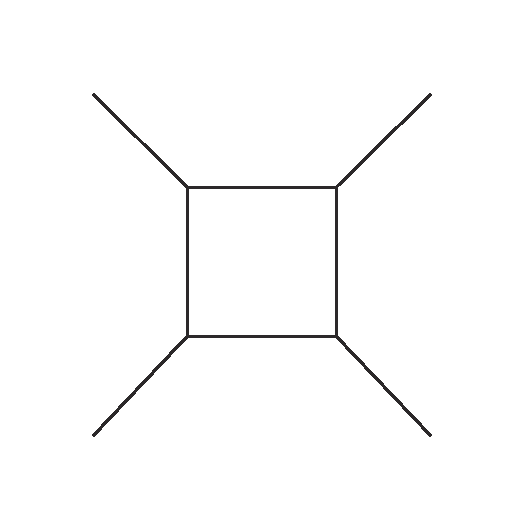
\includegraphics[width=4cm]{Divergence} \hspace{2cm}\includegraphics[width=4cm]{string-loop}
\end{figure}




\vspace{.3cm}
\noindent $\bullet$
Strings besides vibrating in usual spacetime can also have some internal degree of freedom. These internal degrees of freedom are fermionic. This can be quantized in a similar manner to that for bosonic strings. Then, a superstring can be considered as a string that has symmetry between bosonic states and fermionic states. In superstring theories, the good feature (e.g. emergence of gravity and UV finiteness) are preserved, and one can incorporate fermions. Moreover, as mentioned,  the tachyonic mode is absent.
\begin{enumerate}
\item the theory is consistent in 10 spacetime dimensions.
\item there are five fully consistent string theories in $d=10$.

Type IIA, Type IIB, Type I (open+closed string), $E_8\times E_8$ heterotic, $SO(32)$ heterotic

\item Type II theories can have D-branes that accommodate open strings. Type IIA (resp. IIB) has D$p$-branes where $p$ is even (resp. odd), and Type I does D9, D5, D1-branes.


\item Furthermore all the five apparently different string theories have been found to be different limits of the same underlying theory called  M-theory

\item In the low energy scale $\ll1/ \ell_s$, a theory is described by supergravity which combines supersymmetry and general relativity.

\end{enumerate}




\vspace{.3cm}
\noindent $\bullet$  How do we reduce the number of dimensions from 10 to 4? The answer is Kaluza-Klein mechanism/compactification.
If we take the 10-dimensional space of the form $\bR^{1,3}\times M$ where $M$ is a 6-dimensional compact space and its size is much smaller than resolution of most powerful  accelerator $\sim 10^{-17}$cm, then a (9+1)-dimensional theory looks like (3+1)-dimensional.  In fact, in order for a theory to be consistent, $M$ has to be a Calabi-Yau manifold (which admits Ricci-flat metric). More importantly, this extra dimensions give ``room'' to derive the complexity of the real world from a simple setting.












\section{Bosonic string theory}
\subsection*{Notation}
In anticipation of
string theory, we consider $D$-dimensional Minkowski space
${\bR}^{1,D-1}$. Throughout
these notes, we work with signature
%
$$ \eta_{\mu\nu} = {\rm diag}(-1,+1,+1,\ldots,+1)$$
%

\subsection*{Nambu-Goto action}
\begin{wrapfigure}{R}{0.4\textwidth}\centering
\includegraphics[width=4cm]{particle}
\end{wrapfigure}
To begin with, let us recall the case of relativistic point particle
$$
\gamma:\tau\to x^\mu(\tau)\in \bR^{1,D-1}~.
$$
The action of relativistic point particle with mass $m$ is
$$
S=m\int^b_ads=m\int^b_a \Big( -\eta_{\mu\nu}\frac{dx^\mu}{d\tau}\frac{dx^\nu}{d\tau}\Big)^{\frac12}d\tau~.
$$
In a similar fashion, we consider a string
$$
\Sigma:(\tau,\sigma)\to X^\mu(\tau,\sigma)\in \bR^{1,D-1}~.
$$
The analogous action, called the \textbf{Nambu-Goto action}, for the string is given by the area of a string worldsheet $\Sigma$ swept by a string
$$
S_{\textrm{NG}}=T\int_\Sigma \textrm{Area}=T\int_\Sigma d^2\sigma\sqrt{-\det (\g_{ab})}~,\qquad \g_{ab}=\eta_{\mu\nu}\partial_a X^\mu\partial_b X^\nu~
$$
where $(\sigma^0,\sigma^1)=( \tau,\sigma)$, and $T:=1/(2\pi \a')$ is the \textbf{string tension}. The tension is usually defined as mass per unit length.
However, we don't know how to quantize the Nambu-Goto action. Instead, for quantization of string worldsheet, we reformulate the action as follows.


\subsection*{String sigma-model action}
Alternatively, we remove the square root and consider the following action
$$
 S_{\sigma}=\frac T2\int d^2\sigma \sqrt{-\det h}~ h^{ab}\partial_a X^\mu \partial_b X^\nu \eta_{\mu\nu}
$$
which is called the \textbf{string sigma-model action}.\footnote{This action is called the Polyakov action in \cite{Polchinski}. However, according to \cite{BBS}, it was discovered by Brink, Di Vecchia and Howe and by Deser and Zumino several years before Polyakov skillfully used it for path-integral quantization of the string. So let's follow the notation of the progenitor, J.H. Schwarz.} Classically the string sigma-model action is equivalent to the Nambu-Goto action.

\subsection*{Symmetry of $ S_{\sigma}$}
\begin{enumerate}
\item\textbf{$D$-dim spacetime Poincare invariance}

The action is certainly invariant under the Poincare transformation
$$ X^\mu(\sigma)\to \L^\mu{}_\nu X^\nu(\sigma)+V^\mu \qquad \Lambda\in \SO(1,D-1)$$
where $\L$ is a Lorentz transformation and $V$ is the translation.

\item\textbf{Worldsheet diffeomorphism invariance}

Under the re-parametrization
\begin{align}
\wt X^{\mu}(\wt\sigma)&=X^{\mu}(\sigma)\quad \textrm{with}\quad  \wt{\sigma}= \wt{\sigma}(\sigma)~,\cr
\wt h^{ab}&=h^{cd}\frac{\partial\wt\sigma^a}{\partial\sigma^c}\frac{\partial\wt\sigma^b}{\partial \sigma^d}~,\nonumber
\end{align}
the action is invariant $\wt S(X^\m,h_{ab})=\wt S(\wt X^\m,\wt h_{ab})$. We have two parameter family of gauge symmetry.
\item\textbf{Weyl invariance}

The action is also  invariant under the metric $\wt h_{ab}=e^{\phi(\sigma)}h_{ab}$ by an arbitrary function $\phi(\sigma)$. This symmetry is called the \textbf{Weyl symmetry}.

\end{enumerate}

\subsection*{Stress-energy tensor}
The stress-energy tensor is defined by
\begin{align}
T_{ab} &=-\frac{4\pi}{\sqrt{-h}}\,\frac{\partial S}{\partial h^{ab}}\cr
&=-\frac1{\a'} \Big[\partial_a X \partial_b X - \frac12h_{ab}\,\partial_c X \partial^c X\Big]
\end{align}
which satisfies
\begin{align}
\textrm{traceless}:& \qquad T^a{}_a=0\cr
\textrm{conservation}:& \qquad \nabla_a T^{ab}=0
\end{align}
Note that the traceless condition indeed follows from the Weyl invariance (exercise), and  the conservation can be shown by using the equation of motion for $X^\m$ in the following.
\begin{align}
\frac{\partial S}{\partial h^{ab}}=0&\ \to \ T_{ab}=0\cr
\frac{\partial S}{\partial X^\mu}=0&\ \to \ \Delta X_\mu=-\frac{1}{\sqrt{-h}}\partial_a(\sqrt{-h}h^{ab}\partial_b X^\mu)=0
\end{align}



\subsection*{Gauge fixing}
The string sigma-model action $S_\sigma$ is equipped with the symmetries above and we need to fix it for quantization. Physics does not depend on a choice of gauge fixing, but if we choose a clever gauge fixing, our life becomes much easier. Actually, gauge fixing in \cite{BBS} makes our life clearer than that in \cite{Polchinski}, so we use the gauge fixing  in \cite{BBS} as follows.

The metric $h_{ab}$ is a 2$\times$2 symmetric matrix and the woldsheet diffeo invariance tells us that there is a coordinate $\sigma^a$ such that the metric is a diagonal $h_{ab}=e^\omega \eta_{ab}$. Then, the Weyl transformation brings it to the 2d Minkowski metric $\eta_{ab}$. Therefore, one can use $h_{ab}= \eta_{ab}$. If we use the light-cone coordinates on the worldsheet
$$ \sigma^\pm = \tau \pm \sigma\ ,\label{wl}$$
then the metric is written as
$$ds^2=-d\sigma^+d\sigma^-~.$$

However, there are residual transformations that leaves the 2d Minkowski metric $\eta_{ab}$ invariant, which is called \textbf{conformal symmetry}:
$$
\sigma^+\to f(\sigma^+) ~, \qquad \sigma^-\to g(\sigma^-)
$$
with a Weyl transformation simultaneously. To fix the conformal symmetry, we introduce the spacetime light-cone coordinates,
%
$$ X^\pm = \sqrt{\frac{1}{2}}(X^0 \pm X^{D-1}) \ .\label{stlc}$$
%
Then we impose
\be X^+ = x^+ + \a' p^+\,\tau  \ . \label{lcg}~,\ee
which is called \textbf{light-cone gauge}.



\subsection*{Mode Expansions}
After the gauge fixing, the the equations of motion simply read
%
$$ \partial_+\partial_- X^\mu = 0\quad \textrm{where} \quad \partial_\pm =\frac12(\partial_\tau\pm\partial_\sigma)~.$$
%
The most general solution is a factorization of left-moving and right-moving waves
%
\be X^\mu(\sigma,\tau) = X^\mu_L(\sigma^+) + X^\mu_R(\sigma^-)\nonumber\ee
%
for arbitrary functions $X^\mu_L$ and $X^\mu_R$. For a closed string, we impose a periodic condition as
\be X^\mu(\sigma,\tau)=X^\mu(\sigma+2\pi,\tau)\ .\label{periodicity}\ee
%
so that the most general can be expanded in Fourier modes
%
\begin{align}\label{mode}
X^\mu_L(\sigma^+) &= \frac12 x^\mu + \frac12 \a' p^\mu \,\sigma^+ + i\sqrt{\frac{\a'}{2}}\sum_{n\neq 0}
\frac{1}{n}\,\wt{\alpha}_n^\mu\, e^{-in\sigma^+} \ ,\cr
X^\mu_R(\sigma^-) &= \frac12 x^\mu + \frac12 \a' p^\mu \,\sigma^- + i\sqrt{\frac{\a'}{2}}\sum_{n\neq 0}
\frac{1}{n}\,{\alpha}_n^\mu\, e^{-in\sigma^-} \ ,
\end{align}
%
where the reality of $X^\mu$ requires that the coefficients of the Fourier modes obey
%
$${\alpha}_n^\mu= (\alpha^\mu_{-n})^\ast\ \ \ ,\ \ \ \wt{\alpha}_n^\mu=(\wt{\alpha}^\mu_{-n})^\ast\ .\label{realalpha}$$
%
This mode expansion will be very important when we come to the quantum theory. We have to keep in mind that we have to impose  the equation of motion
\be\label{constraints}
T_{--}=(\partial_-X)^2 =0\qquad T_{++}= (\partial_+ X)^2 = 0~.
\ee
We will see the implication of these constraints in the quantum theory.






\subsection*{Quantizations}
The momentum conjugate to $X^\mu$ is defined in this gauge
$$
\Pi_\mu=\frac{\delta S}{\delta (\partial_\tau X^\mu)}=T\; \partial_\tau X^\mu~.
$$
The canonical quantization promotes $X^\mu$ and $\Pi_\mu$ to operators that is subject to
%
\begin{align}
&[X^\mu(\sigma,\tau),\Pi_\nu(\sigma^\prime,\tau)]=i\delta(\sigma-\sigma^\prime)
\,\delta^\mu_{\ \nu} &\ , \cr
&[X^\mu(\sigma,\tau),X^\nu(\sigma^\prime,\tau)] = [\Pi_\mu
(\sigma,\tau),\Pi_\nu(\sigma^\prime,\tau)] = 0&\ .\nonumber\end{align}
%
We translate these into commutation relations for the Fourier modes $x^\mu$, $p^\mu$, ${\alpha}_n^\mu$ and $\wt {\alpha}_n^\mu$. Using the mode expansion, we find (exercise)
%
\be [x^\mu,p_\nu]=i\delta^\mu_{\ \nu} \ \ \ {\rm and}\ \ \
{[}{\alpha}_n^\mu,\alpha_m^\nu{]}=
{[}\wt {\alpha}_n^\mu,\tilde{\alpha}_m^\nu{]}
=n\, \eta^{\mu\nu}\delta_{n+m,\,0}\ ,\label{acom}\ee
Therefore, like harmonic oscillators, the creation operators are $\a_{-n}^{\m},\wt \a_{-n}^{\m}$ and the annihilation operators are $\a_{n}^{\m},\wt \a_{n}^{\m}$ for $n\in\bN$ so that the Hilbert space is spanned by
$$
\a_{-n_1}^{\m_1}\cdots \a_{-n_k}^{\m_k} \wt\a_{-n_1}^{\m_1}\cdots \wt\a_{-n_k}^{\m_k}|k\rangle   \qquad \textrm{where} \qquad p^\m|k\rangle=k^\m|k\rangle~.
$$

Let us consider the implication of the constraints \eqref{constraints}. Using the mode expansions \eqref{mode}, the stress-energy tensor can be expressed as
$$
T_{--}=\a'\sum_n L_ne^{-in\sigma^-} \qquad T_{++}=\a'\sum_n \wt L_ne^{-in\sigma^+}
$$
where
\begin{align}\label{Virasoro}
L_m=\frac12 \sum_{n\neq0} \eta_{\m\n} :\a^\m_{m-n}\a^\n_n: \qquad
\wt L_m=\frac12 \sum_{n\neq0} \eta_{\m\n} :\wt \a^\m_{m-n}\wt \a^\n_n:
\end{align}
with $\a_0^\m=\wt \a_0^\m=\sqrt{\frac{\a'}{2}}p^\m$. We will learn $L_m$ are generators of \textbf{Virasoro algebra}.  According to the normal-ordering $: \ :$ prescription, the lowering operators always appear to the right of the raising operators. However, it is easy to see that the normal ordering matters only in $L_0$ and $\wt L_0$.
Thus, in the quantum theory, the constraint \eqref{constraints} on the stress-energy tensor can be interpreted by
$$L_n| \textrm{phys} \rangle =0 \qquad \wt L_n| \textrm{phys} \rangle =0 \qquad \textrm{for} \quad n>0$$
so that
$$
\langle \textrm{phys}'| L_n | \textrm{phys} \rangle =0 \qquad  \langle \textrm{phys}'| \wt L_n | \textrm{phys} \rangle =0 \qquad \textrm{for} \quad n>0~.
$$




\subsection*{Light-cone quantization}
To see the effect of normal ordering in $L_0$, let us consider the meaning of the light-cone gauge \eqref{lcg} in the quantum theory. It is easy to see that \eqref{lcg} implies
$$
\a_n^+=0 \quad \textrm{for} \quad n\neq0~.
$$
Then, the equation of motion
$$
 2\partial_+X^-\partial_+X^+=\sum_{i=1}^{D-2}\partial_+X^i\partial_+ X^i
$$
tells us
$$
 \alpha^-_n = \sqrt{\frac{1}{2\a'}}\frac{1}{p^+}\sum_{m=-\infty}^{+\infty}\sum_{i=1}^{D-2} \alpha_{n-m}^i\alpha^i_m~.
$$
In particular, for $n=0$, we have
$$
M^2 = 2p^+p^- - \sum_{i=1}^{D-2}p^ip^i = \frac{4}{\a'}\left(\sum_{n>0}\sum_{i=1}^{D-2}  \alpha_{-n}^i\alpha_n^i + \frac{D-2}{2}\sum_{n>0} n\right)
$$
The final term clearly diverges. Fortunately, we have nice regularization of this divergence
\begin{align} \sum_{n=1}^\infty n\  \longrightarrow \ \sum_{n=1}^\infty n e^{-\epsilon n} &= -\frac{\partial}{\partial \epsilon}\sum_{n=1}^\infty e^{-\epsilon n} \nonumber\\ &= -\frac{\partial}{\partial\epsilon} (1-e^{-\epsilon})^{-1} \nonumber\\
% &=& \frac{e^\epsilon}{(e^\epsilon -1)^2} \nonumber\\
&= \frac{1}{\epsilon^2}-\frac{1}{12}+{\cal O}(\epsilon)\nonumber\end{align}
%
Obviously the $1/\epsilon$ piece diverges as $\epsilon\rightarrow 0$. This term should be renormalized
away so that we have
%
$$ \sum_{n=1}^\infty n = -\frac{1}{12} \ .$$
%
Hence, we obtain
\be \label{mass} M^2 = \frac{4}{\a'}\left(N-  \frac{D-2}{24} \right)
= \frac{4}{\a'}\left(\wt{N} - \frac{D-2}{24} \right)
\ ,\ee
where
the number operators are defined by
%
$$ N = \sum_{i=1}^{D-2}\sum_{n>0} \alpha^i_{-n}\alpha_n^i\ \ \  ,\ \ \ \tilde{N} = \sum_{i=1}^{D-2}\sum_{n>0} \tilde{\alpha}^i_{-n}\tilde{\alpha}_n^i \ .\label{nntilde}$$
%
It is easy to see  from \eqref{mass}
\be\label{lmc}
N=\wt N
\ee
which is called the \textbf{level-matching condition}. Moreover, if $D>2$, we have the state with negative [mass]${}^2$ for $N=0=\wt N$ which is called the \textbf{tachyon}.




\subsection*{The First Excited States}

Let us look at the first excited states. The level-matching condition \eqref{lmc} requires us to act both right-  $\alpha^j_{-1}$ and left-moving  $\ol \a_{-1}^i$ creation operator on $|0;k\rangle$ simultaneously. Thus, there are $(D-2)^2$ states at $N=1=\overline N$
\be \alpha_{-1}^i\ol \a_{-1}^j\,|0;k\rangle \ ,\label{first}\ee
whose mass
\be M^2 = \frac{4}{\a'}\left(1-\frac{D-2}{24}\right)\ .\nonumber\ee
It is easy to see that the state is under a representation of the little group $\SO(D-2)\subset \SO(1,D-1)$ and therefore it should be massless. Interestingly, this is only the case if the dimension of spacetime is
\be D=26\ .\label{critical-dim}\ee
This is the critical dimension of the bosonic string. In the following sections, we will see from many different viewpoints that bosonic string theory is consistent only in this critical dimension.


Then, the states \eqref{first} transform in the ${\bf 24}\otimes {\bf 24}$ representation of $\SO(24)$, which decomposes into three irreducible representations:
\begin{align}\label{massless}
\renewcommand\arraystretch{1.2}
 \begin{array}{ll}
  \textrm{Graviton}\  G^{\mu\nu} & \alpha^\mu_{-1}\ol \alpha^\nu_{-1} |0;k \rangle  \quad (\textrm{symmetric in $\mu$ and $\nu$, and traceless} ) \ , \\[2pt]
  \textrm{$B$-field}\ B^{\mu\nu} & \alpha^\mu_{-1}\ol \alpha^\nu_{-1} |0;k \rangle  \quad (\textrm{anti-symmetric in $\mu$ and $\nu$} ) \ , \\[2pt]
  \textrm{Dilaton}\ \Phi & \alpha^\mu_{-1}\ol \alpha_{-1,\mu} |0;k \rangle \ .
 \end{array}
\end{align}
Each irreducible representation gives rise to a massless field in spacetime.
As above, the traceless symmetric, anti-symmetric, and the trace part correspond to the graviton $G_{\mu\nu}$, (Kalb-Ramond) $B$-field $B_{\mu\nu}$, and the dilaton $\Phi$, respectively. Therefore, graviton arises naturally from the quantization of closed strings! These massless fields play a pivotal role throughout the lecture notes.  



\bibliography{string-lecture}
\bibliographystyle{halpha}





%
%\begin{thebibliography}{CDLOGP91}
%
%\bibitem[ABJM08]{Aharony:2008ug}
%O.~Aharony, O.~Bergman, D.~L. Jafferis, and J.~Maldacena.
%\newblock {N=6 superconformal Chern-Simons-matter theories, M2-branes and their
%  gravity duals}.
%\newblock {\em JHEP}, 10:091, 2008, \href{http://arxiv.org/abs/0806.1218}{{\tt
%  arXiv:0806.1218}}.
%
%\bibitem[AGT10]{Alday:2009aq}
%L.~F. Alday, D.~Gaiotto, and Y.~Tachikawa.
%\newblock {Liouville Correlation Functions from Four-dimensional Gauge
%  Theories}.
%\newblock {\em Lett. Math. Phys.}, 91:167--197, 2010,
%  \href{http://arxiv.org/abs/0906.3219}{{\tt arXiv:0906.3219}}.
%
%\bibitem[BBS06]{BBS}
%K.~Becker, M.~Becker, and J.~H. Schwarz.
%\newblock {\em {String theory and M-theory: A modern introduction}}.
%\newblock Cambridge University Press, 2006.
%
%\bibitem[BCH73]{Bardeen:1973gs}
%J.~M. Bardeen, B.~Carter, and S.~W. Hawking.
%\newblock {The Four laws of black hole mechanics}.
%\newblock {\em Commun. Math. Phys.}, 31:161--170, 1973.
%
%\bibitem[Bek72]{bekenstein1972black}
%J.~D. Bekenstein.
%\newblock Black holes and the second law.
%\newblock {\em Lettere Al Nuovo Cimento (1971--1985)}, 4(15):737--740, 1972.
%
%\bibitem[BL07]{Bagger:2006sk}
%J.~Bagger and N.~Lambert.
%\newblock {Modeling Multiple M2's}.
%\newblock {\em Phys. Rev.}, D75:045020, 2007,
%  \href{http://arxiv.org/abs/hep-th/0611108}{{\tt arXiv:hep-th/0611108}}.
%
%\bibitem[BLT13]{Blumenhagen:2013fgp}
%R.~Blumenhagen, D.~Lust, and S.~Theisen.
%\newblock {\em {Basic concepts of string theory}}.
%\newblock Theoretical and Mathematical Physics. Springer, Heidelberg, Germany,
%  2013.
%
%\bibitem[CdLOGP91]{Candelas:1990rm}
%P.~Candelas, X.~C. de~La~Ossa, P.~S. Green, and L.~Parkes.
%\newblock {A Pair of Calabi-Yau manifolds as an exactly soluble superconformal
%  theory}.
%\newblock {\em Nucl. Phys.}, B359:21--74, 1991.
%\newblock [AMS/IP Stud. Adv. Math.9,31(1998)].
%
%\bibitem[Din07]{Dine:2007zp}
%M.~Dine.
%\newblock {\em {Supersymmetry and string theory: Beyond the standard model}}.
%\newblock 2007.
%
%\bibitem[Gai12]{Gaiotto:2009we}
%D.~Gaiotto.
%\newblock {N=2 dualities}.
%\newblock {\em JHEP}, 08:034, 2012, \href{http://arxiv.org/abs/0904.2715}{{\tt
%  arXiv:0904.2715}}.
%
%\bibitem[Gre99]{Greene:1999kj}
%B.~R. Greene.
%\newblock {\em {The elegant universe: Superstrings, hidden dimensions, and the
%  quest of the ultimate theory}}.
%\newblock 1999.
%
%\bibitem[GS84]{Green:1984sg}
%M.~B. Green and J.~H. Schwarz.
%\newblock {Anomaly Cancellation in Supersymmetric D=10 Gauge Theory and
%  Superstring Theory}.
%\newblock {\em Phys. Lett.}, 149B:117--122, 1984.
%
%\bibitem[GSW87]{GSW}
%M.~B. Green, J.~H. Schwarz, and E.~Witten.
%\newblock {\em {Superstring Theory Vol. 1,2}}.
%\newblock Cambridge University Press, 1987.
%
%\bibitem[Haw75]{Hawking:1974sw}
%S.~W. Hawking.
%\newblock {Particle Creation by Black Holes}.
%\newblock {\em Commun. Math. Phys.}, 43:199--220, 1975.
%\newblock [,167(1975)].
%
%\bibitem[Haw76]{Hawking:1976ra}
%S.~W. Hawking.
%\newblock {Breakdown of Predictability in Gravitational Collapse}.
%\newblock {\em Phys. Rev.}, D14:2460--2473, 1976.
%
%\bibitem[Hos15]{Hosomichi}
%K. Hosomichi, \newblock {\em {Lecture notes on string theory}}.
%\newblock 2015
%\href{http://web.phys.ntu.edu.tw/hosomiti/course-string15.html}{{\tt http://web.phys.ntu.edu.tw/hosomiti/course-string15.html}}.
%
%
%\bibitem[IU12]{Ibanez:2012zz}
%L.~E. Ibanez and A.~M. Uranga.
%\newblock {\em {String theory and particle physics: An introduction to string
%  phenomenology}}.
%\newblock Cambridge University Press, 2012.
%
%\bibitem[Mal99]{Maldacena:1997re}
%J.~M. Maldacena.
%\newblock {The Large N limit of superconformal field theories and
%  supergravity}.
%\newblock {\em Int. J. Theor. Phys.}, 38:1113--1133, 1999,
%  \href{http://arxiv.org/abs/hep-th/9711200}{{\tt arXiv:hep-th/9711200}}.
%\newblock [Adv. Theor. Math. Phys.2,231(1998)].
%
%\bibitem[Oog15]{Ooguribook}
%H.~Ooguri.
%\newblock {Superstring theory}.
%\newblock {\em Book for the general public in Chinese}, 2015.
%
%\bibitem[Pol98]{Polchinski}
%J.~Polchinski.
%\newblock {\em {String theory. Vol. 1, 2}}.
%\newblock Cambridge University Press, 1998.
%
%\bibitem[Pol17]{Polchinski:2017vik}
%J.~Polchinski.
%\newblock {Memories of a Theoretical Physicist}.
%\newblock 2017, \href{http://arxiv.org/abs/1708.09093}{{\tt arXiv:1708.09093}}.
%
%\bibitem[RT06]{Ryu:2006bv}
%S.~Ryu and T.~Takayanagi.
%\newblock {Holographic derivation of entanglement entropy from AdS/CFT}.
%\newblock {\em Phys. Rev. Lett.}, 96:181602, 2006,
%  \href{http://arxiv.org/abs/hep-th/0603001}{{\tt arXiv:hep-th/0603001}}.
%
%\bibitem[Sch02]{Schwarz}
%J.~H. Schwarz.
%\newblock {Interview with John H. Schwarz}.
%\newblock {\em Caltech Oral Histories}, 2002.
%
%  \href{http://oralhistories.library.caltech.edu/116/1/Schwarz_OHO.pdf}{{\tt
%  http://oralhistories.library.caltech.edu/116/1/Schwarz\_OHO.pdf}}.
%
%
%
%\bibitem[Sch11]{Schwarz:2011ona}
%J.~H. Schwarz.
%\newblock {The Early History of String Theory and Supersymmetry}.
%\newblock {\em Pontif. Acad. Sci. Scr. Varia}, 119:69--81, 2011,
%  \href{http://arxiv.org/abs/1201.0981}{{\tt arXiv:1201.0981}}.
%
%
%\bibitem[SV96]{Strominger:1996sh}
%A.~Strominger and C.~Vafa.
%\newblock {Microscopic origin of the Bekenstein-Hawking entropy}.
%\newblock {\em Phys. Lett.}, B379:99--104, 1996,
%  \href{http://arxiv.org/abs/hep-th/9601029}{{\tt arXiv:hep-th/9601029}}.
%
%\bibitem[Ton09]{Tong:2009np}
%D.~Tong.
%\newblock {String Theory}.
%\newblock 2009, \href{http://arxiv.org/abs/0908.0333}{{\tt arXiv:0908.0333}}.
%
%\bibitem[Ura05]{Uranga}
%A.~M. Uranga.
%\newblock {Introduction to String Theory}.
%\newblock 2005,
%  \href{http://members.ift.uam-csic.es/auranga/Lect.pdf}{{\tt
%  http://members.ift.uam-csic.es/auranga/Lect.pdf}}.
%
%\bibitem[Ven68]{Veneziano:1968yb}
%G.~Veneziano.
%\newblock {Construction of a crossing - symmetric, Regge behaved amplitude for
%  linearly rising trajectories}.
%\newblock {\em Nuovo Cim.}, A57:190--197, 1968.
%
%\bibitem[Wit94]{Witten:1994cg}
%E.~Witten.
%\newblock {Monopoles and four manifolds}.
%\newblock {\em Math. Res. Lett.}, 1:769--796, 1994,
%  \href{http://arxiv.org/abs/hep-th/9411102}{{\tt arXiv:hep-th/9411102}}.
%
%\bibitem[Wit95]{Witten:1995ex}
%E.~Witten.
%\newblock {String theory dynamics in various dimensions}.
%\newblock {\em Nucl. Phys.}, B443:85--126, 1995,
%  \href{http://arxiv.org/abs/hep-th/9503124}{{\tt arXiv:hep-th/9503124}}.
%
%\bibitem[Zwi06]{Zwiebach:2004tj}
%B.~Zwiebach.
%\newblock {\em {A first course in string theory}}.
%\newblock Cambridge University Press, 2006.
%
%\end{thebibliography}
%
%


\end{document}
